\قسمت{تعریف پروژه}
در این پروژه درسی، سه مقاله از دو مجلهٔ \مل{IEEE Access} و \مل{IEEE Transactions on Neural Networks and Learning Systems} انتخاب شدند. این سه مقاله به گونه‌ای انتخاب شدند که هر سه با استفاده از شبکه‌های عصبی، یک خانواده از کنترل‌کننده‌ها را پیاده‌سازی کرده باشند و هر یک نوآوری‌های متفاوتی داشته باشند. همچنین این سه مقاله از جدید به قدیم، به صورت زنجیره‌ای به یکدیگر ارجاع داده‌اند.

سه مقالهٔ مورد بحث، در سراسر این متن به ترتیب با نام‌های \آ\پانویس{Sakhavi}، \ب\پانویس{Kwon} و \پ\پانویس{Jeong} مورد اشاره قرار گرفته‌اند و شمارهٔ ارجاع آن‌ها به ترتیب \مرجع{Sakhavi2018}، \مرجع{Kwon2020} و \مرجع{Jeong2020} می‌باشد.
\قسمت[مقدمه‌ای بر \مل{BCI}]{مقدمه‌ای بر \مل{BCI}\پانویس{Brain-Computer Interface}}
در یک تعریف رسمی، \مل{BCI} یا واسط مغز-کامپیوتر، به سیستم‌هایی گفته می‌شود که فعالیت سیستم عصبی مرکزی\پانوشت{مغز و نخاع} را اندازه‌گیری کرده و یک خروجی تولید می‌کند که جایگزین کننده یا بازگرداننده یا کامل کننده یا ارتقاء دهندهٔ خروجی طبیعی سیستم عصبی مرکزی بوده و بدین ترتیب تغییراتی را در رابطهٔ سیستم عصبی مرکزی با محیط ایجاد می‌کند \مرجع{Hill2016}.

یک از کاربرد مهم \مل{BCI} در طراحی اندام‌های مصنوعی است؛ به این صورت که از سیگنال‌های عصبی بیماری که دچار مشکلات عصبی-حرکتی است استفاده شده و حرکت یک عضو مصنوعی مکانیکی کنترل می‌شود. در چنین سیستمی، \مل{BCI} به عنوان بخشی از یک سیستم کنترلی مکاترونیکی عمل می‌کند. سه مقالهٔ مورد بررسی در این گزارش نیز روی همین حوزه تمرکز دارند.

ساختار فعالیت‌های مغزی و روش‌های استخراج آن‌ها دامنهٔ وسیعی دارد. ساده‌ترین و رایج‌ترین روش خواندن فعالیت مغزی، روش \مل{EEG}\پانویس{Electroencephalography} می‌باشد. در این روش، با قرار دادن چند الکترود روی سر\پانوشت{روش‌های مشابهی نیز برای نمونه‌برداری از دستگاه عصبی محیطی (مانند عصب‌های روی مچ) وجود دارد.} بیمار، میدان الکتریکی در نقاط مختلف خوانده می‌شود (شکل \رجوع{الکترود}). داده‌ها در روش \مل{EEG} به صورت موج‌های چند کاناله ذخیره می‌شوند و نرخ نمونه برداری دیجیتال\پانویس{Sample rate} معمولا در حد چند صد هرتز است.

\begin{figure}
\centering
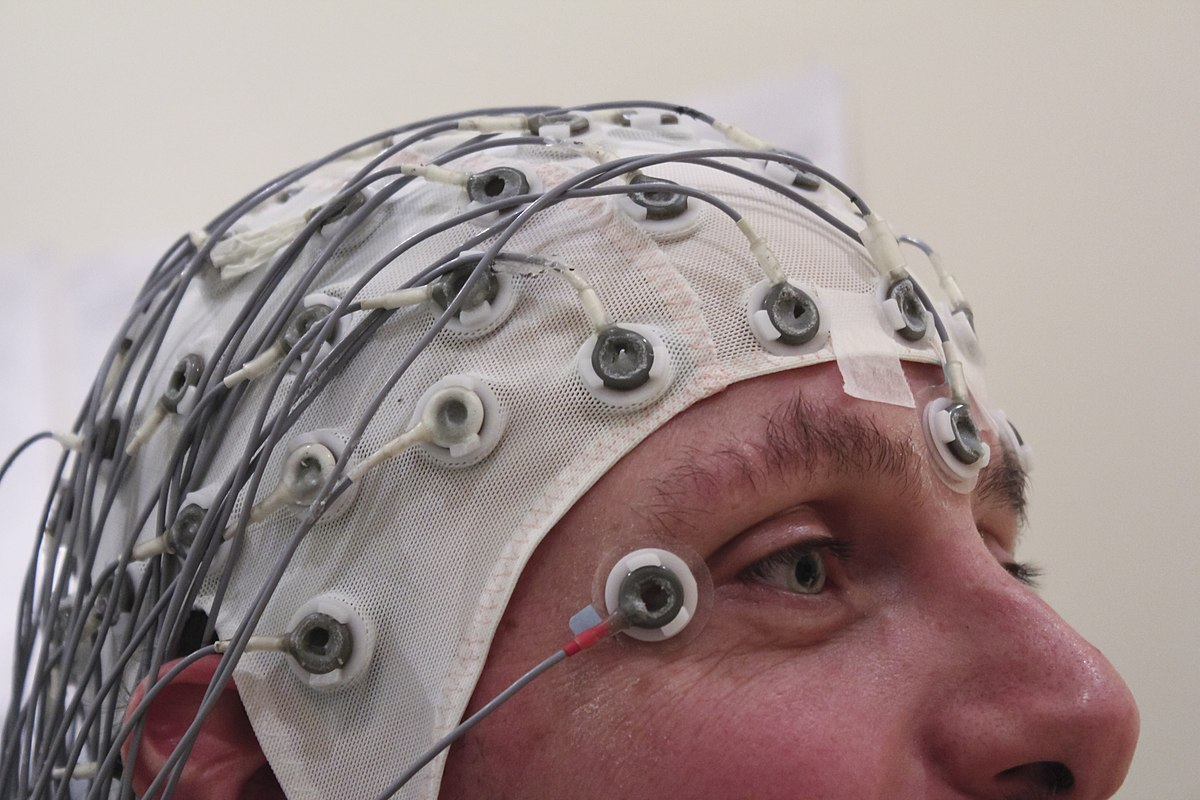
\includegraphics[width=8cm]{img/electrodes.jpg}
\شرح{تجهیزات نمونه‌برداری \مل{EEG} نصب شده روی سر فرد داوطلب \مرجع{Sheerman-Chase2012}}
\برچسب{الکترود}
\end{figure}

\قسمت{مقدمه‌ای بر مقالات مورد بررسی}
مقالات مورد بررسی در این گزارش، از شبکهٔ عصبی کانولوشنال (\مل{CNN})\پانویس{Convolutional Neural Network} برای طبقه‌بندی امواج \مل{EEG} و تشخیص حرکت مورد نظر کاربر استفاده کرده‌اند. این نقطهٔ اشتراک بسیار مهم است زیرا در زمینهٔ طبقه‌بندی امواج، روش‌هایی مانند خوشه‌بندی\پانویس{Clustering}، \مل{LDA}\پانویس{Linear Discriminant Analysis}، \مل{SVM}\پانویس{Support Vector Machine}، \مل{HMM}\پانویس{Hidden Markov Modelling} و... نیز به خوبی مورد استفاده قرار گرفته‌اند \مرجع{Sanei2013}.

تفاوت و نوآوری این مقالات، در دو زمینه هستند: تکنیک‌های پیش‌پردازش\پانویس{Pre-processing}\بالانویس‌متنی{ و }\پانوشت{در این متن، تبدیل فضا (\مل{transformation}) و تهیه نمایش داده (\مل{data representation}) نیز ذیل پیش‌پردازش در نظر گرفته شده‌اند.}
و معماری شبکهٔ عصبی\پانویس{Architecture}. تفاوت‌های ثانویهٔ مقالات مورد بررسی نیز در جزییات اهداف و همچنین دیتاست‌های مورد استفادهٔ آن‌ها می‌باشد.

مقالات مورد بررسی در بخش مربوطه به طور کامل تشریح شده‌اند.

\قسمت{بخش‌های این گزارش}
این گزارش در ۵ فصل تهیه شده است:
\شروع{فقرات}
\فقره[] \متن‌سیاه{فصل ۱ - مقدمه}: فصل حاضر.
\فقره[] \متن‌سیاه{فصل ۲ - تشریح مقالات مورد بررسی}: در این فصل، مقالات مورد بررسی به طور دقیق مورد بررسی قرار گرفته و مقایسه شده اند.
\فقره[] \متن‌سیاه{فصل ۳ - پیاده‌سازی نرم‌افزاری}: در این فصل به الگوها و کتابخانه‌های مورد استفاده برای بازتولید الگوریتم‌های آمده در مقالات اشاره شده است. همچنین در این فصل فهرست فایل‌ها و همچنین راهنمای اجرای کد آمده است.
\فقره[] \متن‌سیاه{فصل ۴ - تحلیل نتایج}: در این فصل نتایج اجرای کد‌ها در قالب نمودارها و جداول آمده است.
\فقره[] \متن‌سیاه{فصل ۵ - بحث و نتیجه‌گیری}: در این فصل با توجه به نتایج به دست آمده، مقالات نقد شده‌اند و پیشنهاداتی نیز آمده است.
\پایان{فقرات}

